% ===================================================================
% DOCUMENTO PRINCIPALE (main.tex) - Versione con Sezioni
% Compila questo file per generare l'intera relazione.
% ===================================================================

\documentclass[12pt, a4paper]{article} % Usa la classe 'article' per documenti basati su sezioni

% --- PACCHETTI GLOBALI NECESSARI ---
\usepackage[utf8]{inputenc}
\usepackage[T1]{fontenc}
\usepackage{graphicx}
\usepackage{xcolor}
\usepackage{listings}
\usepackage{geometry}
\usepackage{times}
\usepackage{caption}
\usepackage[italian]{babel} % Imposta la lingua italiana per sillabazione e nomi
\usepackage{float} % Per un miglior controllo del posizionamento delle figure [H]
\usepackage{tabularx} % Aggiunto per le tabelle con larghezza definita
\usepackage{hyperref} % Rende i riferimenti e l'indice cliccabili

% --- IMPOSTAZIONI DI PAGINA E STILE ---
\geometry{a4paper, top=3cm, bottom=3cm, left=2.5cm, right=2.5cm}
\setlength{\parindent}{0pt} % Rimuove l'indentazione all'inizio dei paragrafi
\setlength{\parskip}{1.5ex} % Aggiunge spazio verticale tra i paragrafi

% --- IMPOSTAZIONE PER I COLLEGAMENTI IPERTESTUALI ---
\hypersetup{
    colorlinks=true,
    linkcolor=black,
    filecolor=magenta,      
    urlcolor=blue,
    citecolor=black,
    pdftitle={Relazione Progetto Ingegneria del Software - JavaBrew},
    pdfpagemode=FullScreen,
}

% --- DEFINIZIONE DELLO STILE PER IL CODICE (TEMA CHIARO) ---
\definecolor{codegreen}{rgb}{0,0.6,0}
\definecolor{codegray}{rgb}{0.5,0.5,0.5}
\definecolor{codepurple}{rgb}{0.58,0,0.82}
\definecolor{codeblue}{rgb}{0,0,0.6}
\definecolor{backcolour}{rgb}{0.95,0.95,0.95}

\lstdefinestyle{vscode_light_style}{
    backgroundcolor=\color{backcolour},   
    commentstyle=\color{codegreen},
    keywordstyle=\color{codeblue},
    numberstyle=\tiny\color{codegray},
    stringstyle=\color{codepurple},
    basicstyle=\fontfamily{pcr}\selectfont\color{black}\small,
    breakatwhitespace=false,         
    breaklines=true,                 
    captionpos=b,                    
    keepspaces=true,                 
    numbers=left,                    
    numbersep=10pt,                  
    showspaces=false,                
    showstringspaces=false,
    showtabs=false,                  
    tabsize=2,
    frame=single,
    framerule=0pt,
    framexleftmargin=5pt,
    framexrightmargin=5pt,
    framextopmargin=5pt,
    framexbottommargin=5pt,
    aboveskip=1.5\baselineskip,
    belowskip=1.5\baselineskip
}

% ===================================================================
% INIZIO DEL DOCUMENTO
% ===================================================================
\begin{document}

% --- INCLUSIONE DEL FRONTESPIZIO ---
% Il file titlePage.tex conterra' \maketitle e le informazioni del titolo/autore
\input{titlePage.tex}

% --- INDICE DEI CONTENUTI ---
% Questo comando genera automaticamente l'indice basandosi sui comandi \section e \subsection
\tableofcontents
\newpage

% --- INCLUSIONE DELLE SEZIONI ---
% Ogni sezione e' in un file separato.
% Assicurati che ogni file .tex inizi con \section{...}

% Ordine richiesto:
\input{introduction.tex}
\input{useCases.tex}
% --- INIZIO SEZIONE DATABASE ---
% Questo file contiene solo il contenuto per questa sezione
% e viene incluso dal file main.tex

\section{Progettazione del Database}

La persistenza dei dati è un requisito fondamentale per l'applicazione \textbf{JavaBrew}, in quanto garantisce che tutte le informazioni relative a utenti, macchine, prodotti e transazioni siano conservate in modo sicuro e coerente. Per soddisfare questa esigenza, è stato progettato un database relazionale, il cui schema è stato definito attraverso un modello Entità-Relazione (ER). Questa sezione illustra la struttura logica del database, descrivendo le entità principali, i loro attributi e le relazioni che le legano.

\subsection{Schema Entità-Relazione (ER)}

Il diagramma ER, mostrato nella Figura \ref{fig:er_diagram}, fornisce una visione d'insieme completa della struttura del database. Questo modello è stato la guida per la creazione delle tabelle fisiche e per l'implementazione del livello di persistenza (DAO) nell'applicazione. Il design segue i principi di normalizzazione per ridurre la ridondanza dei dati e garantire l'integrità referenziale attraverso l'uso di chiavi primarie e chiavi esterne.

\begin{figure}[h!]
    \centering
    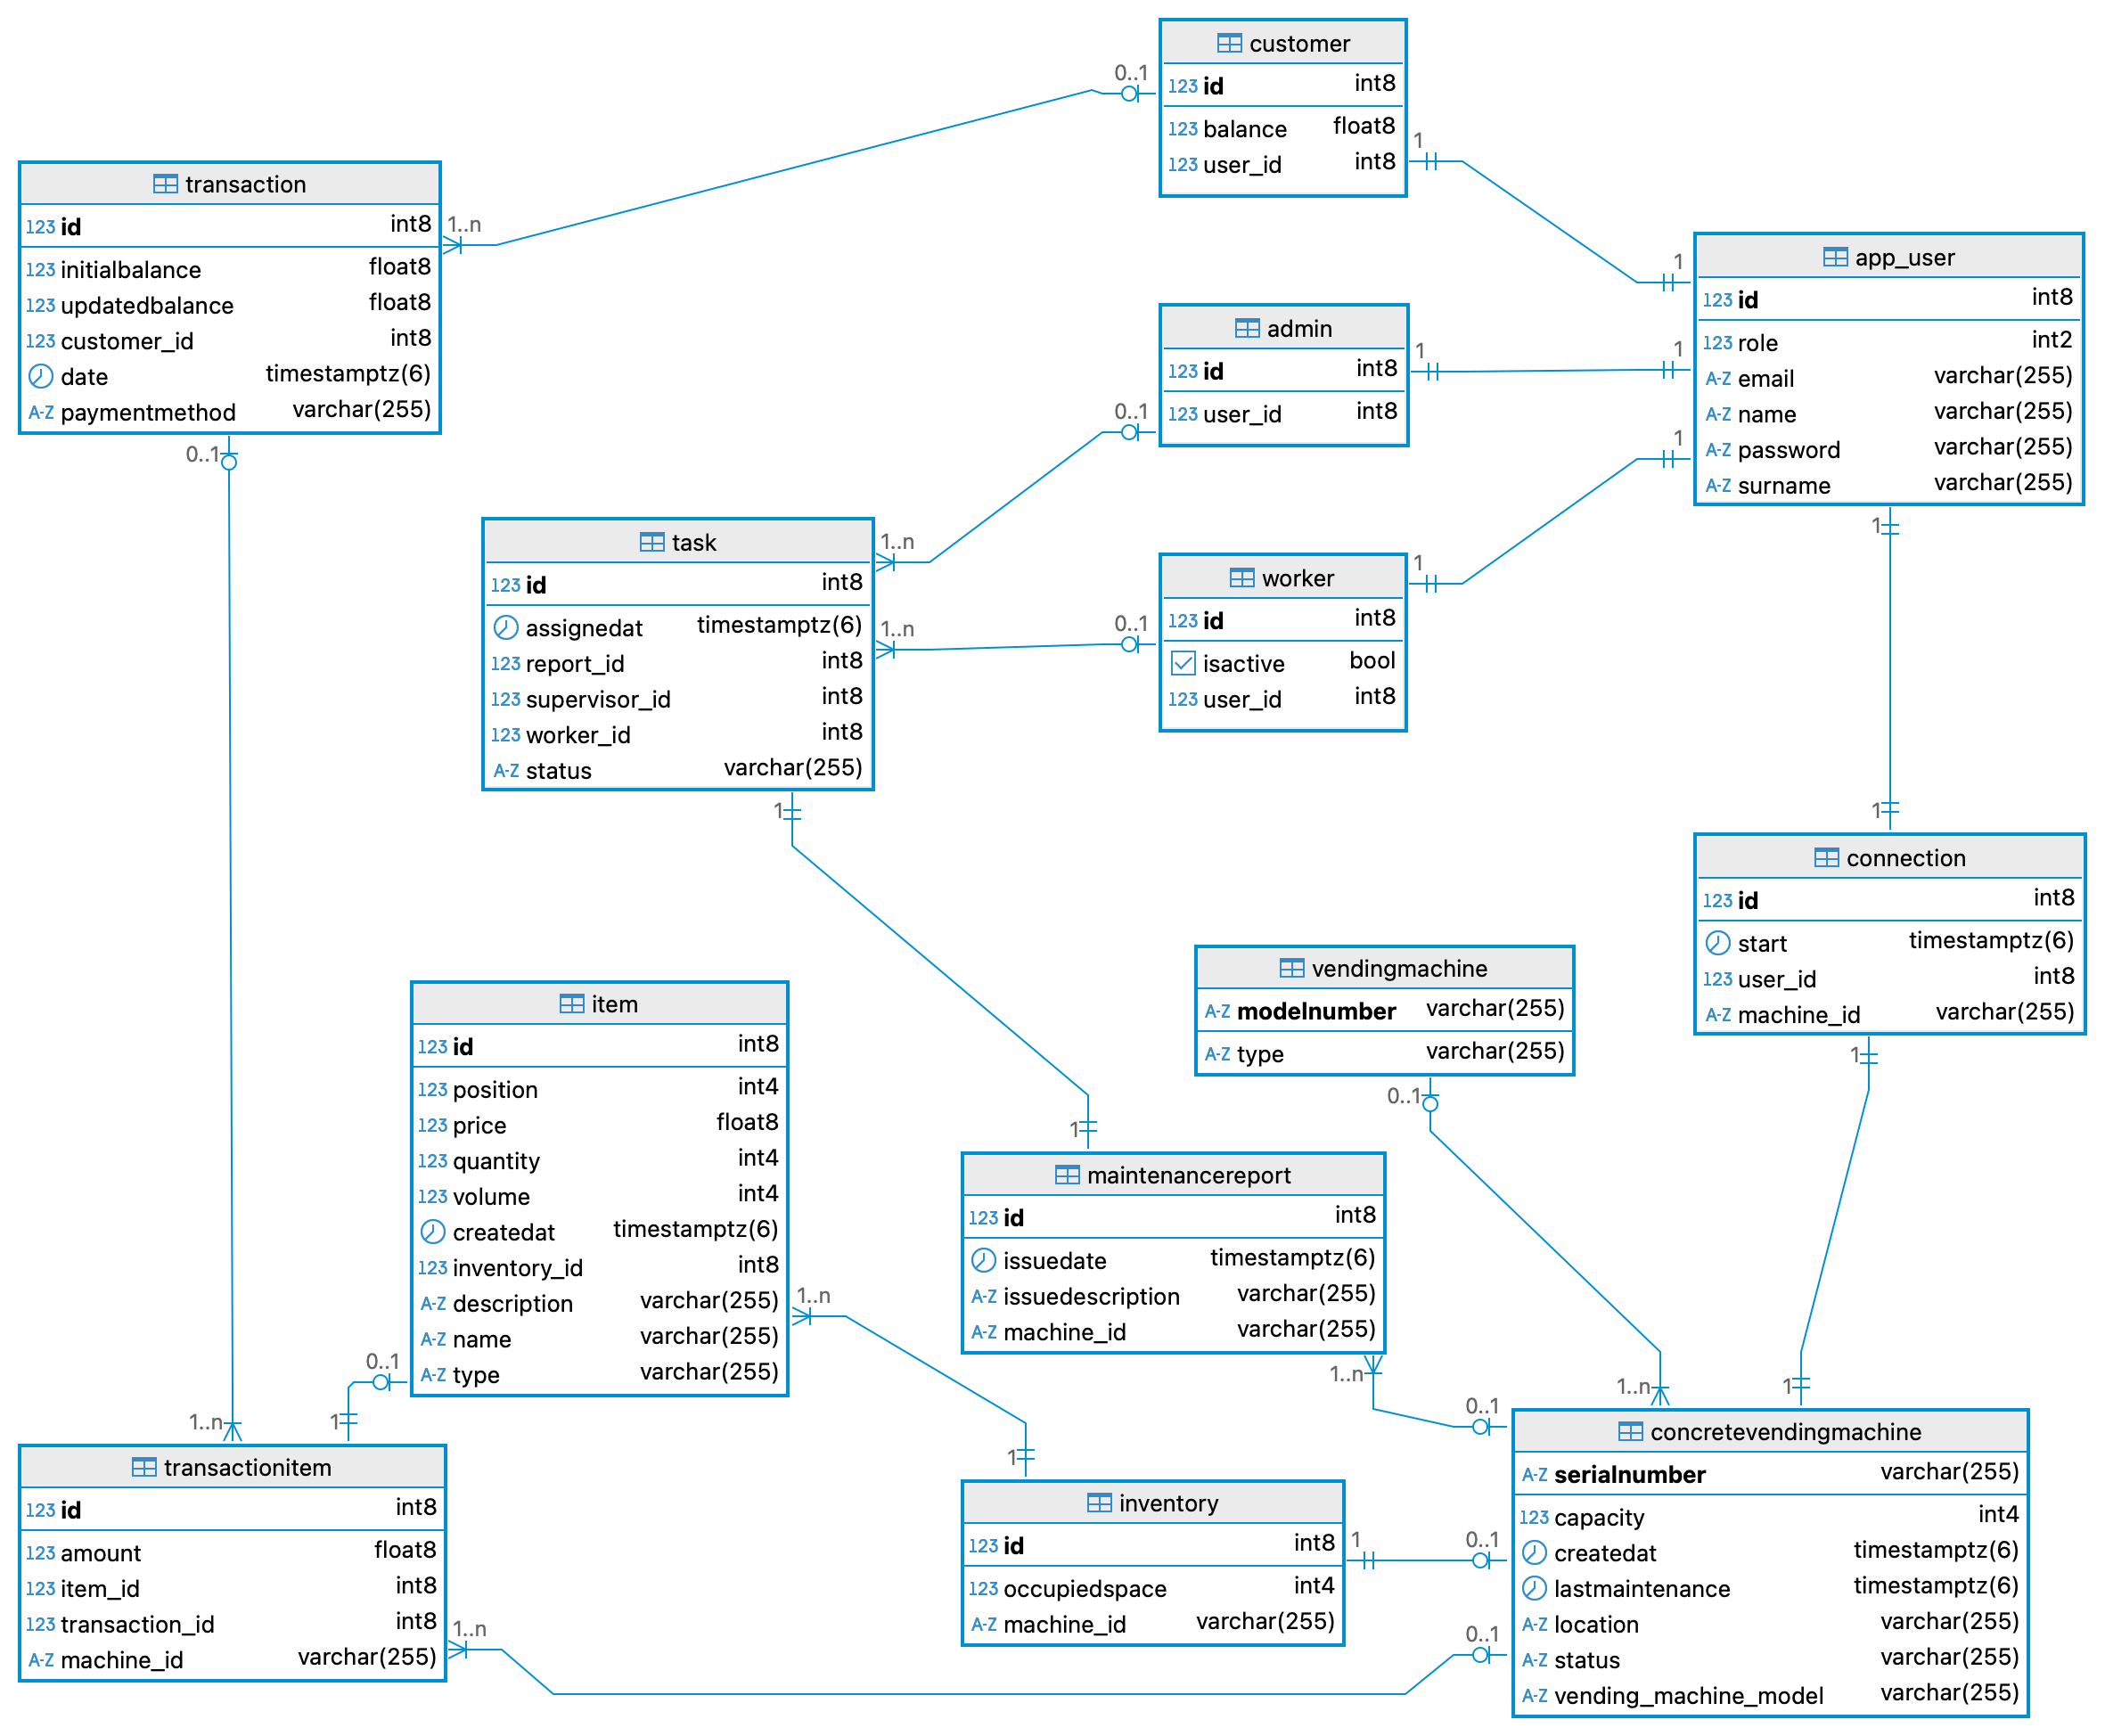
\includegraphics[width=\textwidth]{schemas/ER_Schema.png} 
    \caption{Diagramma Entità-Relazione (ER) del database di JavaBrew.}
    \label{fig:er_diagram}
\end{figure}

\subsection{Analisi Dettagliata delle Tabelle}

Lo schema è organizzato attorno a quattro aree funzionali principali: la gestione degli utenti, la gestione delle macchine, la registrazione delle transazioni e la gestione delle operazioni di manutenzione.

\subsubsection{Gestione degli Utenti}
La modellazione degli utenti adotta un approccio di \textbf{specializzazione}. Esiste una tabella base, \texttt{app\_user}, che contiene gli attributi comuni a tutti i tipi di utente.
\begin{itemize}
    \item \textbf{\texttt{app\_user}}: Funge da genitore e memorizza le informazioni anagrafiche e di accesso fondamentali, come \texttt{id}, \texttt{email}, \texttt{password}, \texttt{name}, \texttt{surname} e \texttt{role}. Il campo \texttt{role} è cruciale per distinguere le diverse tipologie di utente.
    \item \textbf{\texttt{customer}}, \textbf{\texttt{admin}}, \textbf{\texttt{worker}}: Sono tabelle di specializzazione. Ognuna ha una relazione uno-a-uno con \texttt{app\_user}, identificata dalla chiave esterna \texttt{user\_id}. Questo design permette di estendere gli attributi specifici per ogni ruolo. Ad esempio, la tabella \texttt{customer} contiene il campo \texttt{balance} per il credito, mentre la tabella \texttt{worker} ha un flag \texttt{isactive}.
\end{itemize}

\subsubsection{Gestione delle Macchine e dell'Inventario}
Anche la modellazione delle macchine da caffè segue un principio di specializzazione, separando il concetto generico di macchina da quello concreto e installato.
\begin{itemize}
    \item \textbf{\texttt{vendingmachine}}: Tabella che definisce i modelli generici di macchina, con attributi come \texttt{modelnumber} e \texttt{type}.
    \item \textbf{\texttt{concretevendingmachine}}: Rappresenta un'istanza fisica di una macchina installata in un determinato luogo. È collegata a un modello generico tramite la chiave esterna \texttt{vending\_machine\_model} e possiede attributi operativi come \texttt{serialnumber}, \texttt{location}, \texttt{status} e \texttt{capacity}.
    \item \textbf{\texttt{inventory}}: Ogni macchina concreta ha un inventario (relazione uno-a-uno). La tabella \texttt{inventory} tiene traccia dello spazio occupato (\texttt{occupiedspace}) e funge da collegamento per gli articoli.
    \item \textbf{\texttt{item}}: Contiene l'elenco dei prodotti disponibili, con attributi come \texttt{name}, \texttt{price}, \texttt{quantity} e \texttt{position}. È collegata all'inventario di una specifica macchina tramite la chiave esterna \texttt{inventory\_id}.
\end{itemize}

\subsubsection{Gestione delle Transazioni}
Questa area è responsabile della tracciabilità di tutte le operazioni finanziarie.
\begin{itemize}
    \item \textbf{\texttt{transaction}}: Memorizza l'intestazione di una transazione, come l'acquisto o una ricarica. Include l'ID del cliente (\texttt{customer\_id}), il metodo di pagamento (\texttt{paymentmethod}), e il bilancio iniziale e finale (\texttt{initialbalance}, \texttt{updatedbalance}) per una facile verifica.
    \item \textbf{\texttt{transactionitem}}: Tabella di dettaglio che realizza la relazione molti-a-molti tra transazioni e articoli. Ogni record rappresenta una riga di uno scontrino, collegando un \texttt{transaction\_id} a un \texttt{item\_id} e specificando l'importo (\texttt{amount}).
\end{itemize}

\subsubsection{Gestione Operativa}
Questo gruppo di tabelle supporta le operazioni quotidiane dell'applicazione.
\begin{itemize}
    \item \textbf{\texttt{connection}}: Traccia le connessioni attive tra un cliente e una macchina, memorizzando \texttt{user\_id}, \texttt{machine\_id} e l'orario di inizio (\texttt{start}).
    \item \textbf{\texttt{task}} e \textbf{\texttt{maintenancereport}}: Supportano il flusso di lavoro dei tecnici. Un \texttt{task} (compito) viene assegnato a un \texttt{worker} e può generare un \texttt{maintenancereport} (rapporto di manutenzione) una volta completato.
\end{itemize}

\subsection{Scelte Progettuali e Integrità dei Dati}

La progettazione del database è stata guidata da due principi chiave: la \textbf{normalizzazione} e l'\textbf{integrità referenziale}.
\begin{itemize}
    \item \textbf{Normalizzazione}: Lo schema è stato progettato per raggiungere almeno la Terza Forma Normale (3NF), riducendo al minimo la ridondanza dei dati. Ad esempio, le informazioni di un utente sono memorizzate una sola volta nella tabella \texttt{app\_user}, evitando duplicazioni.
    \item \textbf{Integrità Referenziale}: L'uso estensivo di chiavi esterne (foreign key) garantisce che le relazioni tra le tabelle siano sempre valide. Ad esempio, non è possibile creare una transazione per un cliente che non esiste, o assegnare un compito a un tecnico non presente nel sistema. Questi vincoli, imposti a livello di database, proteggono i dati da inconsistenze e sono fondamentali per la robustezza dell'intera applicazione.
\end{itemize}
 
\input{mockups.tex}
% --- INIZIO SEZIONE IMPLEMENTAZIONE E TESTING ---
% Questo file contiene solo il contenuto per questa sezione
% e viene incluso dal file main.tex

\section{Implementazione e Testing}

La presente sezione illustra le scelte implementative, le tecnologie adottate e le strategie di testing impiegate per lo sviluppo dell'applicazione \textbf{JavaBrew}. L'implementazione ha seguito i modelli di progettazione delineati nella fase di analisi, come evidenziato dai diagrammi UML, e si è avvalsa di un insieme di tecnologie mature per garantire robustezza, manutenibilità e testabilità del sistema software.

\subsection{Architettura del Sistema e Stack Tecnologico}

Il progetto è stato sviluppato utilizzando \textbf{Java 17} e gestito tramite \textbf{Apache Maven} per l'automazione del build process. L'architettura software è stata strutturata in un approccio a livelli, promuovendo una chiara separazione delle responsabilità tra i componenti. I livelli principali, conformemente alla documentazione UML, comprendono:
\begin{itemize}
\item \textbf{Livello Controller:} Interfaccia diretta con l'utente, responsabile della gestione delle richieste e dell'invocazione della logica di business.
\item \textbf{Livello Service:} Contiene la logica di business primaria dell'applicazione. Orchestrazione delle operazioni, elaborazione dei dati e interazione con il livello di persistenza.
\item \textbf{Livello DAO (Data Access Object):} Gestisce l'interazione con il database, fornendo un'astrazione completa dei dettagli di persistenza dei dati.
\item \textbf{Livello Model:} Definisce le entità del dominio, rappresentando la struttura dei dati all'interno del sistema.
\end{itemize}

---

\subsection{Livello di Persistenza: Pattern DAO e ORM Hibernate}

La persistenza dei dati è stata implementata adottando il pattern \textbf{Data Access Object (DAO)}. Tale approccio prevede la definizione di interfacce (es. \texttt{UserDao}) e relative implementazioni concrete (es. \texttt{UserDaoImpl}), consentendo il disaccoppiamento della logica di business dalle specifiche tecnologie di persistenza.

Per l'interazione con il database relazionale, è stato utilizzato \textbf{Hibernate ORM} (versione 6.5.2), un framework per l'Object-Relational Mapping. L'adozione di Hibernate, in congiunzione con l'API standard \textbf{Jakarta Persistence (JPA)}, ha permesso di astrarre la scrittura di codice SQL nativo, facilitando il mapping diretto degli oggetti Java del modello su tabelle del database. Il database di produzione selezionato è \textbf{PostgreSQL}.

La gestione delle connessioni al database è centralizzata nella classe \texttt{DBManager}. Questa classe opera come un singleton statico, fornendo un punto di accesso globale e univoco all'\texttt{EntityManagerFactory}, l'oggetto responsabile della creazione di \texttt{EntityManager} per le operazioni sul database.

\begin{lstlisting}[language=Java, style=vscode_light_style, caption={La classe \texttt{DBManager} per la gestione dell'accesso all'EntityManagerFactory di JPA.}]
package com.smartvend.app.db;

import jakarta.persistence.EntityManagerFactory;
import jakarta.persistence.Persistence;

public class DBManager {
    private static EntityManagerFactory emf;
    // ... Altri campi e metodi ...
    
    public static EntityManagerFactory getEntityManagerFactory() {
        if (emf == null) {
            init(); % Assicura che l'EMF sia inizializzato se richiesto
        }
        return emf;
    }
    // ... Metodo shutdown ...
}
\end{lstlisting}

---

\subsection{Livello di Logica di Business (Service Layer)}

Il livello Service incapsula la logica applicativa core. Ciascun servizio (es. \texttt{CustomerService}) dipende dalle interfacce DAO per l'accesso ai dati, aderendo al principio di \textbf{Inversione delle Dipendenze}. Il metodo \texttt{buyItem} esemplifica l'orchestrazione delle operazioni di business: recupero delle entità, applicazione delle regole di business (validazione del saldo e della disponibilità dei prodotti), aggiornamento dello stato del sistema (quantità e saldo) e registrazione della transazione.

\begin{lstlisting}[language=Java, style=vscode_light_style, caption={Estratto del metodo \texttt{buyItem} dalla classe \texttt{CustomerService}.}]
public Transaction buyItem(long connectionId, List<Long> itemIds) {
    // 1. Recupera la connessione e il cliente
    Connection connection = connectionDao.getConnectionById(connectionId);
    // ... controlli null ...
    Customer customer = customerDao.getCustomerByUserId(connection.getUserId());
    // ... controlli null ...

    // 2. Calcola il prezzo totale e valida la disponibilita' degli articoli
    double totalPrice = 0.0;
    List<Item> itemsToUpdate = new ArrayList<>();
    for (Long itemId : itemIds) {
        Item item = itemDao.getItemById(itemId);
        // ... controlli disponibilità ...
        totalPrice += item.getPrice();
        itemsToUpdate.add(item);
    }

    // 3. Controlla il saldo del cliente PRIMA di ogni modifica
    double initialBalance = checkBalance(customer.getId(), totalPrice);

    // 4. Se il saldo e' sufficiente, aggiorna lo stato del sistema
    for (Item item : itemsToUpdate) {
        item.setQuantity(item.getQuantity() - 1);
        itemDao.updateItem(item);
    }
    updateBalance(customer.getId(), totalPrice);

    // 5. Crea e registra la transazione
    Transaction transaction = new Transaction(
            customer, PaymentMethod.Wallet, initialBalance, 
            initialBalance - totalPrice, createTransactionItems(itemsToUpdate));

    return transactionService.createTransaction(transaction);
}
\end{lstlisting}

---

\subsection{Ambiente di Esecuzione con Docker}

Per assicurare un ambiente di sviluppo e di esecuzione riproducibile e consistente, il database \textbf{PostgreSQL} è stato containerizzato tramite \textbf{Docker}. La containerizzazione, in questo contesto, offre diversi vantaggi: garantisce la \textbf{parità tra gli ambienti} di sviluppo, test e produzione, mitigando le problematiche di "funzionamento solo sulla macchina locale". Inoltre, \textbf{isola le dipendenze}, racchiudendo il database e le relative librerie all'interno del container, prevenendo interferenze con altri servizi o software sull'host. L'impiego di un file \texttt{docker-compose.yml} per la definizione del servizio funge da "Infrastructure as Code", documentando e versionando l'ambiente necessario per l'applicazione e semplificando la configurazione per i nuovi membri del team.

---

\subsection{Strategia di Testing}

La qualità del software è stata validata attraverso una strategia di testing strutturata, che ha incluso sia \textbf{test di unità} sia \textbf{test di integrazione}. Questo approccio a livelli è essenziale per verificare il sistema da diverse prospettive: la correttezza logica dei singoli componenti e la loro corretta interazione all'interno dell'architettura. Gli strumenti configurati nel file \texttt{pom.xml} hanno permesso di automatizzare e validare il funzionamento del codice a vari livelli.

\subsubsection{Test di Unità e Mocking}

I test di unità sono stati sviluppati con \textbf{JUnit 5} per verificare l'isolamento e la correttezza funzionale dei singoli componenti. Per testare il livello Service in assenza di dipendenza dal livello di persistenza, è stato utilizzato il framework di mocking \textbf{Mockito}. Questo ha consentito di simulare il comportamento dei DAO (tramite l'annotazione \texttt{@Mock}) e di iniettarli nel servizio sotto test (tramite \texttt{@InjectMocks}), focalizzando l'analisi esclusivamente sulla logica di business. Tale isolamento è cruciale per l'esecuzione rapida dei test (centinaia di test in pochi secondi, senza latenza del database) e per la verifica deterministica di ogni percorso logico e caso limite del servizio.

\begin{lstlisting}[language=Java, style=vscode_light_style, caption={Esempio semplificato di test unitario per il metodo \texttt{buyItem} con JUnit 5 e Mockito.}]
public class CustomerServiceTest {
    @Mock private CustomerDaoImpl customerDao;
    @Mock private ItemDaoImpl itemDao;
    @Mock private TransactionService transactionService;
    @InjectMocks private CustomerService customerService;

    private Customer mockCustomer;
    private Item mockItem1;

    @BeforeEach
    public void setUp() {
        MockitoAnnotations.openMocks(this);
        mockCustomer = new Customer(2L, new User(1L, "...", "Jhon", "Doe", "..."), 100.0);
        mockItem1 = new Item(30L, "Soda", "...", 1, 10, 1.50, 3, ItemType.Bottle);
    }
    
    @Test
    @DisplayName("Test buyItem method success with single item")
    void testBuyItemSuccessSingleItem() {
        // Arrange: Prepara i dati e il comportamento dei mock
        % ... definizione mockConnection e expectedTransaction (commentate perché non direttamente nel codice) ...
        when(itemDao.getItemById(30L)).thenReturn(mockItem1);
        when(transactionService.createTransaction(any(Transaction.class))).thenReturn(expectedTransaction);

        // Act: Esegui il metodo da testare
        Transaction result = customerService.buyItem(1L, List.of(30L));

        // Assert: Verifica il risultato e le interazioni con i mock
        assertNotNull(result);
        assertEquals(9, mockItem1.getQuantity()); 
        verify(itemDao, times(1)).updateItem(mockItem1);
        verify(customerDao, times(1)).updateCustomer(mockCustomer);
        verify(transactionService, times(1)).createTransaction(any(Transaction.class));
    }
}
\end{lstlisting}

\subsubsection{Test di Integrazione}

I test di integrazione sono stati implementati per verificare la corretta interazione tra i vari livelli dell'applicazione, in particolare tra il Service Layer, il DAO Layer e il database. Per questi test, è stato impiegato un database in-memory \textbf{H2}, che ha permesso l'esecuzione dell'intero stack di persistenza in un ambiente controllato e ad alta velocità. Questi test sono fondamentali per identificare problematiche non rilevabili dai test di unità, quali errori nelle annotazioni di mapping JPA, gestione delle transazioni, o incompatibilità con il dialetto SQL specifico di PostgreSQL. La validazione di tali interazioni in un ambiente controllato, prima del deployment, costituisce un passaggio critico per la robustezza del sistema.

\subsubsection{Analisi della Copertura del Codice}

Per monitorare l'efficacia e la completezza della suite di test, è stato integrato il plugin \textbf{JaCoCo} in Maven. L'esecuzione congiunta dei test di unità e di integrazione ha permesso di conseguire e mantenere una \textbf{copertura del codice superiore all'80\%}. Questo risultato quantitativo fornisce una metrica oggettiva della qualità del software, attestando che la maggior parte della logica implementata è stata verificata tramite test automatici. L'analisi della copertura, inoltre, supporta l'identificazione di "codice morto" (porzioni di codice mai eseguite) e assicura che i percorsi logici critici, inclusi quelli relativi alla gestione degli errori, siano stati adeguatamente testati, contribuendo al miglioramento continuo della qualità.

\begin{figure}[h!]
    \centering % Centra l'immagine nella pagina
    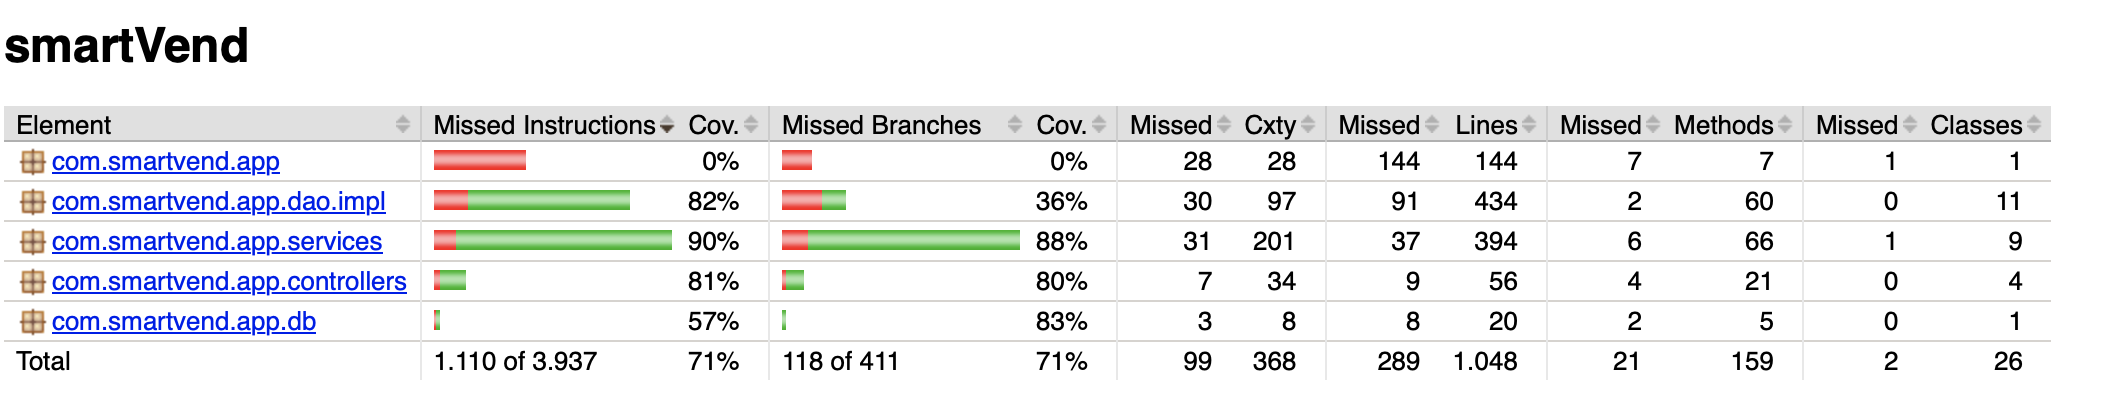
\includegraphics[width=0.8\textwidth]{assets/coverage.png} % Specifica il percorso e il nome del file immagine
    % 'width=0.8\textwidth' imposta la larghezza all'80% della larghezza del testo. Regola se necessario.
    \caption{Riepilogo della copertura del codice per package (generato da JaCoCo).} % Didascalia dell'immagine
    \label{fig:jacoco_coverage} % Etichetta per riferimenti incrociati nel testo (es. "come mostrato in Figura \ref{fig:jacoco_coverage}")
\end{figure}
% --- Fine del codice per l'immagine del coverage ---

\end{document}
